\documentclass{ximera}

\outcome{Calculate limits of the form number over zero.}
\outcome{Identify determinate and indeterminate forms.}
\outcome{Distinguish between determinate and indeterminate forms.}

%\usepackage{todonotes}

\newcommand{\todo}{}

\usepackage{tkz-euclide}
\tikzset{>=stealth} %% cool arrow head
\tikzset{shorten <>/.style={ shorten >=#1, shorten <=#1 } } %% allows shorter vectors

\usepackage{tkz-tab}  %% sign charts
\usetikzlibrary{decorations.pathreplacing} 

\usetikzlibrary{backgrounds} %% for boxes around graphs
\usetikzlibrary{shapes,positioning}  %% Clouds and stars
\usetikzlibrary{matrix} %% for matrix
\usepgfplotslibrary{polar} %% for polar plots
\usetkzobj{all}
\usepackage[makeroom]{cancel} %% for strike outs
%\usepackage{mathtools} %% for pretty underbrace % Breaks Ximera
\usepackage{multicol}

\usepackage{polynom}



\usepackage[many]{tcolorbox}  %% for titled boxes
\newtcolorbox{xbox}[1]{%
    tikznode boxed title,
    enhanced,
    arc=0mm,
    interior style={white},
    attach boxed title to top center= {yshift=-\tcboxedtitleheight/2},
    fonttitle=\bfseries,
    colbacktitle=white,coltitle=black,
    boxed title style={size=normal,colframe=white,boxrule=0pt},
    title={#1}}


\usepackage{array}
\setlength{\extrarowheight}{+.1cm}   
\newdimen\digitwidth
\settowidth\digitwidth{9}
\def\divrule#1#2{
\noalign{\moveright#1\digitwidth
\vbox{\hrule width#2\digitwidth}}}





\newcommand{\RR}{\mathbb R}
\newcommand{\R}{\mathbb R}
\newcommand{\N}{\mathbb N}
\newcommand{\Z}{\mathbb Z}

%\renewcommand{\d}{\,d\!}
\renewcommand{\d}{\mathop{}\!d}
\newcommand{\dd}[2][]{\frac{\d #1}{\d #2}}
\newcommand{\pp}[2][]{\frac{\partial #1}{\partial #2}}
\renewcommand{\l}{\ell}
\newcommand{\ddx}{\frac{d}{\d x}}
\newcommand{\ddt}{\frac{d}{\d t}}

\newcommand{\zeroOverZero}{\ensuremath{\boldsymbol{\tfrac{0}{0}}}}
\newcommand{\inftyOverInfty}{\ensuremath{\boldsymbol{\tfrac{\infty}{\infty}}}}
\newcommand{\zeroOverInfty}{\ensuremath{\boldsymbol{\tfrac{0}{\infty}}}}
\newcommand{\zeroTimesInfty}{\ensuremath{\small\boldsymbol{0\cdot \infty}}}
\newcommand{\inftyMinusInfty}{\ensuremath{\small\boldsymbol{\infty - \infty}}}
\newcommand{\oneToInfty}{\ensuremath{\boldsymbol{1^\infty}}}
\newcommand{\zeroToZero}{\ensuremath{\boldsymbol{0^0}}}
\newcommand{\inftyToZero}{\ensuremath{\boldsymbol{\infty^0}}}



\newcommand{\numOverZero}{\ensuremath{\boldsymbol{\tfrac{\#}{0}}}}
\newcommand{\dfn}{\textbf}
%\newcommand{\unit}{\,\mathrm}
\newcommand{\unit}{\mathop{}\!\mathrm}
\newcommand{\eval}[1]{\bigg[ #1 \bigg]}
\newcommand{\seq}[1]{\left( #1 \right)}
\renewcommand{\epsilon}{\varepsilon}
\renewcommand{\iff}{\Leftrightarrow}

\DeclareMathOperator{\arccot}{arccot}
\DeclareMathOperator{\arcsec}{arcsec}
\DeclareMathOperator{\arccsc}{arccsc}
\DeclareMathOperator{\si}{Si}
\DeclareMathOperator{\proj}{proj}
\DeclareMathOperator{\scal}{scal}


\newcommand{\tightoverset}[2]{% for arrow vec
  \mathop{#2}\limits^{\vbox to -.5ex{\kern-0.75ex\hbox{$#1$}\vss}}}
\newcommand{\arrowvec}[1]{\tightoverset{\scriptstyle\rightharpoonup}{#1}}
\renewcommand{\vec}{\mathbf}
\newcommand{\veci}{\vec{i}}
\newcommand{\vecj}{\vec{j}}
\newcommand{\veck}{\vec{k}}
\newcommand{\vecl}{\boldsymbol{\l}}

\newcommand{\dotp}{\bullet}
\newcommand{\cross}{\boldsymbol\times}
\newcommand{\grad}{\boldsymbol\nabla}
\newcommand{\divergence}{\grad\dotp}
\newcommand{\curl}{\grad\cross}
%\DeclareMathOperator{\divergence}{divergence}
%\DeclareMathOperator{\curl}[1]{\grad\cross #1}


\colorlet{textColor}{black} 
\colorlet{background}{white}
\colorlet{penColor}{blue!50!black} % Color of a curve in a plot
\colorlet{penColor2}{red!50!black}% Color of a curve in a plot
\colorlet{penColor3}{red!50!blue} % Color of a curve in a plot
\colorlet{penColor4}{green!50!black} % Color of a curve in a plot
\colorlet{penColor5}{orange!80!black} % Color of a curve in a plot
\colorlet{fill1}{penColor!20} % Color of fill in a plot
\colorlet{fill2}{penColor2!20} % Color of fill in a plot
\colorlet{fillp}{fill1} % Color of positive area
\colorlet{filln}{penColor2!20} % Color of negative area
\colorlet{fill3}{penColor3!20} % Fill
\colorlet{fill4}{penColor4!20} % Fill
\colorlet{fill5}{penColor5!20} % Fill
\colorlet{gridColor}{gray!50} % Color of grid in a plot

\newcommand{\surfaceColor}{violet}
\newcommand{\surfaceColorTwo}{redyellow}
\newcommand{\sliceColor}{greenyellow}




\pgfmathdeclarefunction{gauss}{2}{% gives gaussian
  \pgfmathparse{1/(#2*sqrt(2*pi))*exp(-((x-#1)^2)/(2*#2^2))}%
}


%%%%%%%%%%%%%
%% Vectors
%%%%%%%%%%%%%

%% Simple horiz vectors
\renewcommand{\vector}[1]{\left\langle #1\right\rangle}


%% %% Complex Horiz Vectors with angle brackets
%% \makeatletter
%% \renewcommand{\vector}[2][ , ]{\left\langle%
%%   \def\nextitem{\def\nextitem{#1}}%
%%   \@for \el:=#2\do{\nextitem\el}\right\rangle%
%% }
%% \makeatother

%% %% Vertical Vectors
%% \def\vector#1{\begin{bmatrix}\vecListA#1,,\end{bmatrix}}
%% \def\vecListA#1,{\if,#1,\else #1\cr \expandafter \vecListA \fi}

%%%%%%%%%%%%%
%% End of vectors
%%%%%%%%%%%%%

%\newcommand{\fullwidth}{}
%\newcommand{\normalwidth}{}



%% makes a snazzy t-chart for evaluating functions
%\newenvironment{tchart}{\rowcolors{2}{}{background!90!textColor}\array}{\endarray}

%%This is to help with formatting on future title pages.
\newenvironment{sectionOutcomes}{}{} 



%% Flowchart stuff
%\tikzstyle{startstop} = [rectangle, rounded corners, minimum width=3cm, minimum height=1cm,text centered, draw=black]
%\tikzstyle{question} = [rectangle, minimum width=3cm, minimum height=1cm, text centered, draw=black]
%\tikzstyle{decision} = [trapezium, trapezium left angle=70, trapezium right angle=110, minimum width=3cm, minimum height=1cm, text centered, draw=black]
%\tikzstyle{question} = [rectangle, rounded corners, minimum width=3cm, minimum height=1cm,text centered, draw=black]
%\tikzstyle{process} = [rectangle, minimum width=3cm, minimum height=1cm, text centered, draw=black]
%\tikzstyle{decision} = [trapezium, trapezium left angle=70, trapezium right angle=110, minimum width=3cm, minimum height=1cm, text centered, draw=black]


\title[Dig-In:]{Limits of the form nonzero over zero}

\begin{document}
\begin{abstract}
  We want to solve limits that have the form nonzero over zero.
\end{abstract}

\maketitle

Let's cut to the chase:

\begin{definition}
  A limit
  \[
  \lim_{x\to a} \frac{f(x)}{g(x)}
  \]
  is said to be of the form \numOverZero\ if
  \[
  \lim_{x\to a} f(x) = k\qquad\text{and}\qquad \lim_{x\to a} g(x) =0.
  \]
  where $k$ is some nonzero constant.
\end{definition}

\begin{question}
  Which of the following limits are of the form \numOverZero?
  \begin{selectAll}
    \choice[correct]{$\lim_{x\to -1} \frac{1}{(x+1)^2}$}
    \choice{$\lim_{x\to 2}\frac{x^2-3x+2}{x-2}$}
%    \choice{$\lim_{x\to 0}\frac{\sin(x)}{x}$}
    \choice[correct]{$\lim_{x\to 2}\frac{x^2-3x-2}{x-2}$}
    \choice[correct]{$\lim_{x\to 1}\frac{x}{\sqrt{x}-1}$}
  \end{selectAll}
\end{question}


Let's see what is going on with limits of the form \numOverZero.
Consider the function
  \[
  f(x) = \frac{1}{(x+1)^2}.
  \]
While the $\lim_{x\to -1} f(x)$ does not exist, something can still be
said. First note that
\[
\lim_{x\to -1} \frac{1}{(x+1)^2}\qquad\text{is of the form }\numOverZero
\]
as
\[
\lim_{x\to -1} 1 = 1 \qquad\text{and}\qquad \lim_{x\to -1}(x+1)^2 = 0.
\]
Moreover, as $x$ approaches $-1$:
\begin{itemize}
\item The numerator is positive.
\item The denominator approaches zero and is positive.
\end{itemize}
Hence
\[
\lim_{x\to -1} \frac{1}{(x+1)^2}
\]
will become arbitrarily large, as we can see in the next graph.
\begin{image}
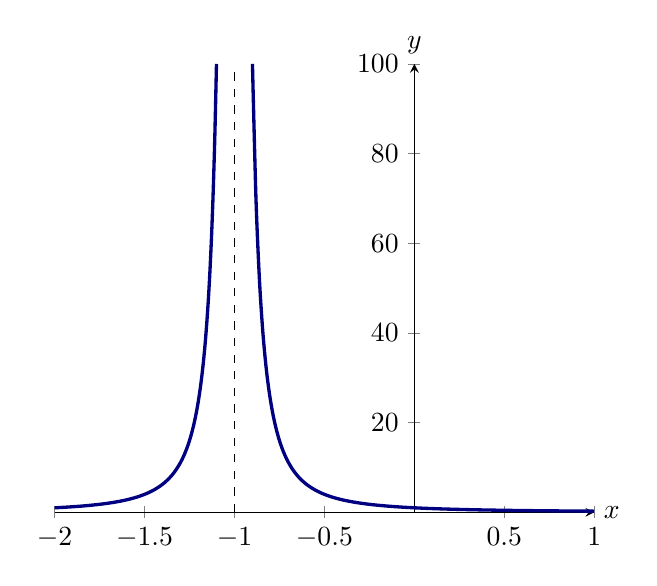
\begin{tikzpicture}
	\begin{axis}[
            domain=-2:1,
            ymax=100,
            samples=100,
            axis lines =middle, xlabel=$x$, ylabel=$y$,
            every axis y label/.style={at=(current axis.above origin),anchor=south},
            every axis x label/.style={at=(current axis.right of origin),anchor=west}
          ]
	  \addplot [very thick, penColor, smooth, domain=(-2:-1.1)] {1/(x+1)^2};
          \addplot [very thick, penColor, smooth, domain=(-.9:1)] {1/(x+1)^2};
          \addplot [textColor, dashed] plot coordinates {(-1,0) (-1,100)};
        \end{axis}
\end{tikzpicture}
\end{image}

We are now ready for our next definition.

\begin{definition}
If $f(x)$ grows arbitrarily large as $x$ approaches $a$, we write
\[
\lim_{x\to a} f(x) = \infty
\]
and say that the limit of $f(x)$ \dfn{approaches infinity} as $x$
goes to $a$.

If $|f(x)|$ grows arbitrarily large as $x$ approaches $a$ and $f(x)$ is
negative, we write
\[
	\lim_{x\to a} f(x) = -\infty
\]
and say that the limit of $f(x)$ \textbf{approaches negative infinity}
as $x$ goes to $a$.
\end{definition}

Let's consider a few more examples.

\begin{example}
  Compute:
  \[
	  \lim_{x\to -2} \frac{5-x}{(x+2)^4}
  \]
  \begin{explanation}
    First let's look at the form of this limit, we do this by taking the limits of both the numerator and denominator:
    \[
    \lim_{x\to -2} 5-x = \answer[given]{7}\qquad\text{and}\lim_{x\to-2}\left((x+2)^4\right) = 0
    \]
    so this limit is of the form \numOverZero.  As $x$ approaches $-2$:
    \begin{itemize}
	    \item The numerator is a \wordChoice{\choice[correct]{positive}\choice{negative}} number. 
	    \item The denominator is \wordChoice{\choice[correct]{positive}\choice{negative}} and is approaching zero.
    \end{itemize}
    This means that
    \[
	    \lim_{x\to -2} \frac{5-x}{(x+2)^4} = \infty.
    \]
  \end{explanation}
\end{example}


\begin{example}
  Compute:
  \[
  \lim_{x\to 3^+} \frac{x^2-9x+14}{x^2-5x+6}
  \]
  \begin{explanation}
    First let's look at the form of this limit, which we do by taking the limits of both the numerator and denominator.
    \[
    \lim_{x\to 3^+} \left(x^2-9x+14\right) = \answer[given]{-4}\qquad\text{and}\lim_{x\to3^+}\left(x^2-5x+6\right) = 0
    \]
    This limit is of the form \numOverZero. Next, we should factor the numerator and denominator to see if we can simplify the problem at all. 
    \begin{align*}
      \lim_{x\to 3^+}\frac{x^2-9x+14}{x^2-5x+6} &= \lim_{x\to 3^+}\frac{(x-2)(x-7)}{(x-2)(x-3)}\\
      &= \lim_{x\to 3^+}\frac{x-7}{x-3}
    \end{align*}
    Canceling a factor of $x-2$ from the numerator and denominator
    means we can more easily check the behavior of this limit.  As $x$
    approaches $3$ from the right:
    \begin{itemize}
    \item The numerator is a \wordChoice{\choice{positive}\choice[correct]{negative}} number. 
    \item The denominator is \wordChoice{\choice[correct]{positive}\choice{negative}} and approaching zero.
    \end{itemize}
    This means that
    \[
    \lim_{x\to 3^+} \frac{x^2-9x+14}{x^2-5x+6} = -\infty.
    \]
   \end{explanation}
\end{example}

Here is our final example.

\begin{example}
  Compute:
  \[
  \lim_{x\to 3} \frac{x^2-9x+14}{x^2-5x+6}
  \]
  \begin{explanation}
    We've already considered part of this example, but now we consider the two-sided limit. We already know that
    \[
    \lim_{x\to 3} \frac{x^2-9x+14}{x^2-5x+6} = \lim_{x\to
      3}\frac{x-7}{x-3},
    \]
    and that this limit is of the form \numOverZero.
    We also know that as $x$ approaches $3$ from the right,
    \begin{itemize}
    \item The numerator is a negative number. 
    \item The denominator is positive and approaching zero.
    \end{itemize}
    Hence our function is approaching $-\infty$ from the right.
    
    As $x$ approaches $3$ from the left,
    \begin{itemize}
    \item The numerator is negative.
    \item The denominator is negative and approaching zero.
    \end{itemize}
    Hence our function is approaching $\infty$ from the left.
    This means
    \[
    \lim_{x\to 3} \frac{x^2-9x+14}{x^2-5x+6} = \answer[given]{DNE}.
    \]
    \begin{onlineOnly}
     We can confirm our results of the previous two examples by looking at the graph of $y=\frac{x^2-9x+14}{x^2-5x+6}$:
     \[
     \graph[xmin=-10,xmax=15,ymin=-10,ymax=10]{\frac{x^2-9x+14}{x^2-5x+6}}
     \]
   \end{onlineOnly}
  \end{explanation}
\end{example}

Some people worry that the mathematicians are passing into mysticism
when we talk about infinity and negative infinity. However, when we write
\[
\lim_{x\to a} f(x) = \infty \qquad\text{and}\qquad \lim_{x\to a} g(x) = -\infty
\]
all we mean is that as $x$ approaches $a$, $f(x)$ becomes arbitrarily
large and $|g(x)|$ becomes arbitrarily large, with $g(x)$ taking
negative values.
\end{document}
